\documentclass[12pt, letterpaper]{article}
\usepackage{graphicx}
\usepackage{hyperref}
\usepackage{amssymb}
\usepackage{amsmath}
\usepackage{float}
\usepackage{mathtools}
\usepackage{enumitem}
\usepackage[margin=1in]{geometry}
\usepackage[figurename=Figura]{caption}

\title{%
  Situación Problema: Análisis de Audio usando Fourier \\
  \large F1009: Análisis de métodos matemáticos para la física}

\begin{document}

\maketitle

\begin{tabular}{ccc}
Juan Pablo Guerrero Escudero & Romina Nájera Fuentes & Juan Braulio Olivares Rodríguez
\end{tabular}

\section{Introducción}

\section{Teoría}

\subsection{Conceptos físicos}

\subsubsection{Ondas de sonido}
De acuerdo a Young y Freedman \cite{university-physics}, El sonido se define como una onda 
longitudinal en un medio, principalmente aire, pero puede ser otros como otros gases, líquidos o sólidos. Las 
ondas de sonido más simple son ondas sinusoidales con una frecuencia, amplitud y longitud definida. 
\cite{university-physics}. El ser humano es capaz de escuchar ondas en el rango de 20 a 20,000 Hz, con 
frecuencias por encima del rango (ultrasónicas) o debajo del rango (infrasónicas) fuera del rango de escucha humano. 
De acuerdo a Hwaitat \cite{frequencies-wave-sound-pso}, las ondas de sonido son peturbancias propagadas por un medio el cuál 
no se ve afectado, y éstas ondas pueden ser ya sea longitudinales, o transversales. Para una onda 
de tipo longitudinal, el medio vibra en ángulos rectos al movimiento de la onda, y en el caso de ondas longitudinales, 
el medio vibra en la misma dirección que el movimiento.En la Figura \ref*{Ondas Longitudinales} se observa gráficamente lo discutido. 
\begin{figure}[H]
  \centering
  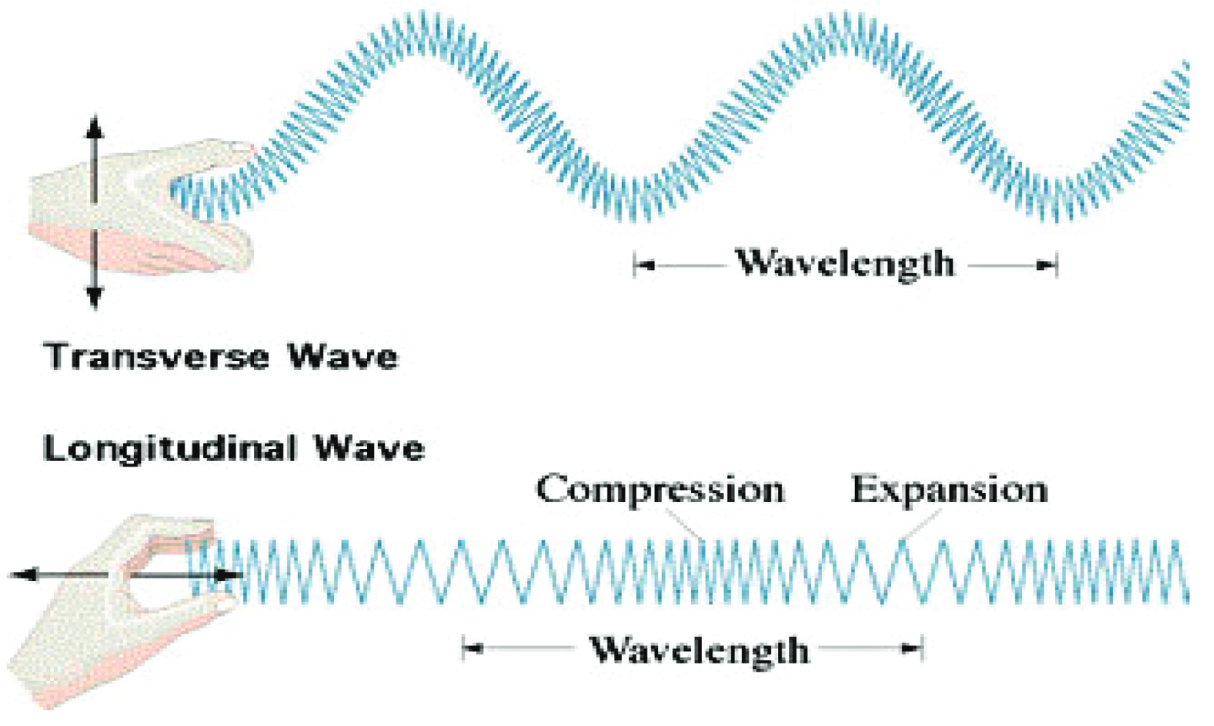
\includegraphics[height = 4cm]{ondas_longitudinales_transversales.png}
  \caption{Ondas longitudinales y transversales}
  \label{Ondas Longitudinales}
\end{figure}
Los parámetros de cualquier onda constituyen la amplitud, la frecuencia 
y la longitud, mencionados anteriormente. La amplitud puede ser definida como la "altura" 
de la onda, la frecuencia se define como los ciclos por segundo, y la longitud se define como la distancia 
entre un pico de onda y otro. Para una vista gráfica, vea la Figura \ref*{parametros-ondas}. Generalmente, sucede que 
cuando dos partículas están en movimiento en el mismo medio, ocurre interferencia. Ésto significa que 
las amplitudes de onda son sumadas algebraicamente, y se siguen moviendo por el medio sin distracciones. En el mundo real, 
la interferencia de ondas crea patrones complejo, y puede ser muy difícil de analizar.  
\begin{figure}[H]
  \centering
  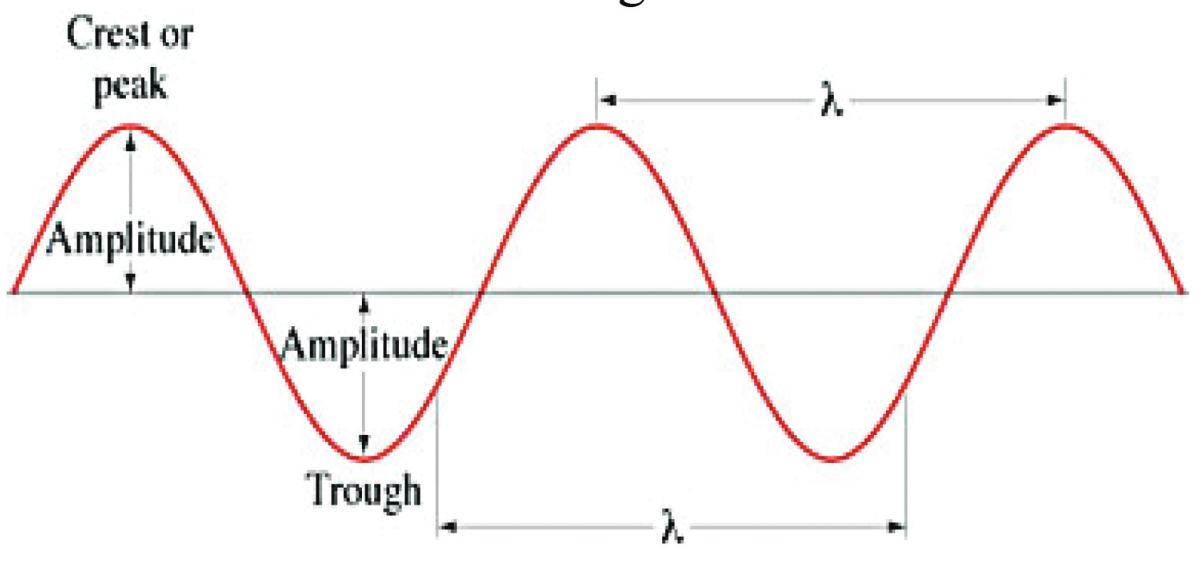
\includegraphics[height = 4cm]{parametros-ondas.png}
  \caption{Parámetros de las ondas de sonido}
  \label{parametros-ondas}
\end{figure}
\subsubsection{Frecuencias de audio/sonido}
Como se definió anteriormente, la frecuencia de una onda es, de acuerdo a \cite{university-physics}, como el número de repeticiones 
    de una función periódica durante una unidad de variación en la variable independiente. En otras palabras, es el número de 
    ocurrencias de un evento repetitivo por unidad de tiempo. Matemáticamente, se dice que en medios no dispersivos (medios donde 
    la velocidad de la onda es independiente de la frecuencia), la frecuencia tiene una relación inversa con la longitud 
    de onda, en la forma de la ecuación \ref{frequency-eq}, donde $\lambda$ es la longitud de la onda, y $v$ es la velocidad de la onda.
    \begin{align}
    f = \frac{v}{\lambda}
    \label{frequency-eq}
    \end{align}Analizando la ecuación \ref{frequency-eq}, observamos que ondas de longitud más corta ($\lambda$), 
    tienen mayores variaciones en la frecuencia debido a que los máximos y mínimos están más cerca uno del otro, y viceversa. Una vista gráfica 
    se observa en la Figura \ref{frecuencias-onda}. 
    \begin{figure}[H]
      \centering
      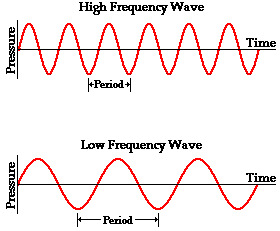
\includegraphics[height = 6cm]{frecuencias-ondas.jpg}
      \caption{Diferentes frecuencias de onda}
      \label{frecuencias-onda}
    \end{figure}
    Además, la frecuencia se mide en Hz o Hertz, equivalente a un evento de repetición por segundo. De acuerdo a \cite{university-physics}, 
    la frecuencia de una onda de sonido es el factor primario al determinar el tono de un sonido. Frecuencias 
    más altas emiten sonidos con mayor tono que frecuencias más bajas. En conjunto, cuando se juntan diferentes frecuencias 
    al mismo tiempo, se crean patrones más complejos que ondas simples sinusoidales, debido a que físicamente, las variaciones en presión 
    del medio que se generan son más complejas. 
\subsubsection{Sonidos armónicos}De acuerdo a \cite{university-physics}, puede suceder que dos tonos producidos por diferentes instrumentos tengan la 
misma frecuencia pero suenen diferente, y ésto es debido a la diferencia en contenido armónico, que está definido como la colección de diferentes frecuencias 
que componen un sonido complejo formado por muchas frecuencias fundamentales. Además, de acuerdo a \cite{university-physics}, otro factor que determina los 
sonidos armónicos de un sonido es el comportamiento al inicio (attack) y al final (decay) de cada tono. Cada instrumento posee una diferente dinámica de sonidos armónicos, 
lo cuál entrega ondas en una mezcla diferente de frecuencias, que da su sonido característico. \\

Para dar algunos ejemplos \cite{orchestra-frecuency}, la nota de afinación en una orquesta sinfónica es A4, que tiene una frecuencia de 440Hz. Frecuencias más complejas se generan cuando 
se utiliza el concepto de octavas en música, que de acuerdo a \cite{octave-definition}, es una serie de 8 notas musicales que ocupan el intervalo entre 2 notas, una teniendo el doble 
o la mitad de la frecuencia que la otra. Es decir, un salto de una octava corresponde a duplicar la frecuencia de la onda de sonido. 
\subsubsection{Beats}
En la física, sucede que cuando se tienen dos ondas con igual amplitud pero ligeramente diferentes frecuencias, si ambas ondas van hacia la 
misma dirección, pasa que en ciertos momentos, las dos ondas están en la misma fase, es decir, sus máximos coinciden y sus amplitudes se suman. Sin embargo, 
debido a que las ondas están en ligeramente distintas frecuencias, llega a haber momentos en los que estas ondas están 
exactamente fuera de fase, y se cancelan una con otra. La variación de amplitud causa variaciones en el volumen, llamadas \textit{beats}, y la frecuencia 
con la que éstos varían se le llama frecuencia de beat. En la Figura \ref{beats-grafica} se muestra éste proceso de manera gráfica.
\begin{figure}[H]
  \centering
  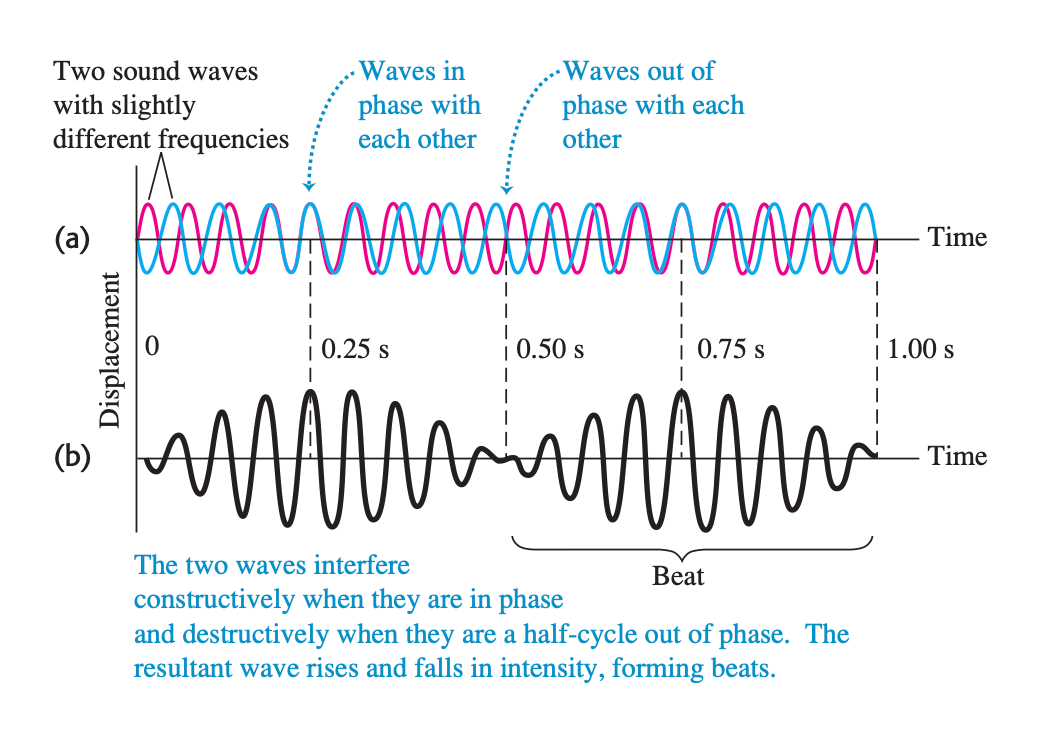
\includegraphics[height = 7cm]{beats-grafica.png}
  \caption{Gráfica del proceso de beats}
  \label{beats-grafica}
\end{figure}Los beats entre dos tonos, de acuerdo a \cite{university-physics}, pueden ser escuchados hasta una frecuencia de beat de 6 o 7Hz. En la práctica, 
una técnica importante es escuchar los beats para afinar los instrumentos musicales. Además, de acuerdo a \cite{university-physics}, cuando las diferencias de 
frecuencia son mayores a 7Hz, se dejan de escuchar beats individuales, y las frecuencias se mezclan en una de consonancia o disonancia, dependiendo de la 
naturaleza de las frecuencias. 
\subsection{Análisis de las canciones}

Para la clasificación de las canciones entre los géneros de música instrumental o reggaetón,
realizaremos un análisis espectral, el cual busca descomponer una serie de tiempo en las
ondas senoidales que la conforman \cite{Montenegro-2009}. Este análisis permitirá obtener las
diferentes frecuencias que conforman al pedazo de canción a analizar, y poder sacar conclusiones
sobre el género de la canción. \medskip

\noindent Para ello, utilizaremos la transformada de Fourier, utilizada
comúnmente en el campo científico, como en la acústica y el procesamiento de señales.
Esta herramienta transforma el dominio de una señal, pasando del tiempo a la frecuencia,
sin alterar su contenido \cite{Bernal-1999}.
Al perderse la noción del tiempo, analizaremos los rangos de frecuencias en los
que se encuentran magnitudes más grandes, para así identificar si la canción presentada
es instrumental o reggaetón.

\subsubsection{Transformada de Fourier}

Por definición, la transformada de Fourier de una función $f(x)$ es dada por la ecuación \ref{eq:fourier}
\begin{align}
	\phi_f(\alpha) &= \int_{-\infty}^{\infty} e^{i\alpha x} f(x) dx
	\label{eq:fourier}
\end{align}

\noindent Esta transformada fue desarrollada por Jean-Baptiste Joseph Fourier en el siglo XIX,
quien inició proponiendo que cualquier función arbitraria de una variable
podía ser expresada como una combinación lineal de funciones de senos y cosenos,
que son las series de Fourier \cite{OGorman-2023}. \medskip

\noindent A través de esas series, logró sintetizar la transformada, la cual
es distinguida por:
\begin{itemize}
  \item Determinar qué frecuencias están presentes en una señal.
  \item Transformar una señal del dominio temporal al dominio de frecuencia y viceversa.
\end{itemize}

\noindent Así como las series de Fourier descomponen una función en senos y cosenos, la
transformada descompone una señal en sus frecuencias, y aquellas que tengan una mayor
amplitud, se verán representadas como picos más altos, así como se puede observar en
la figura \ref{fig:fourier}.

\begin{figure}[H]
  \centering
  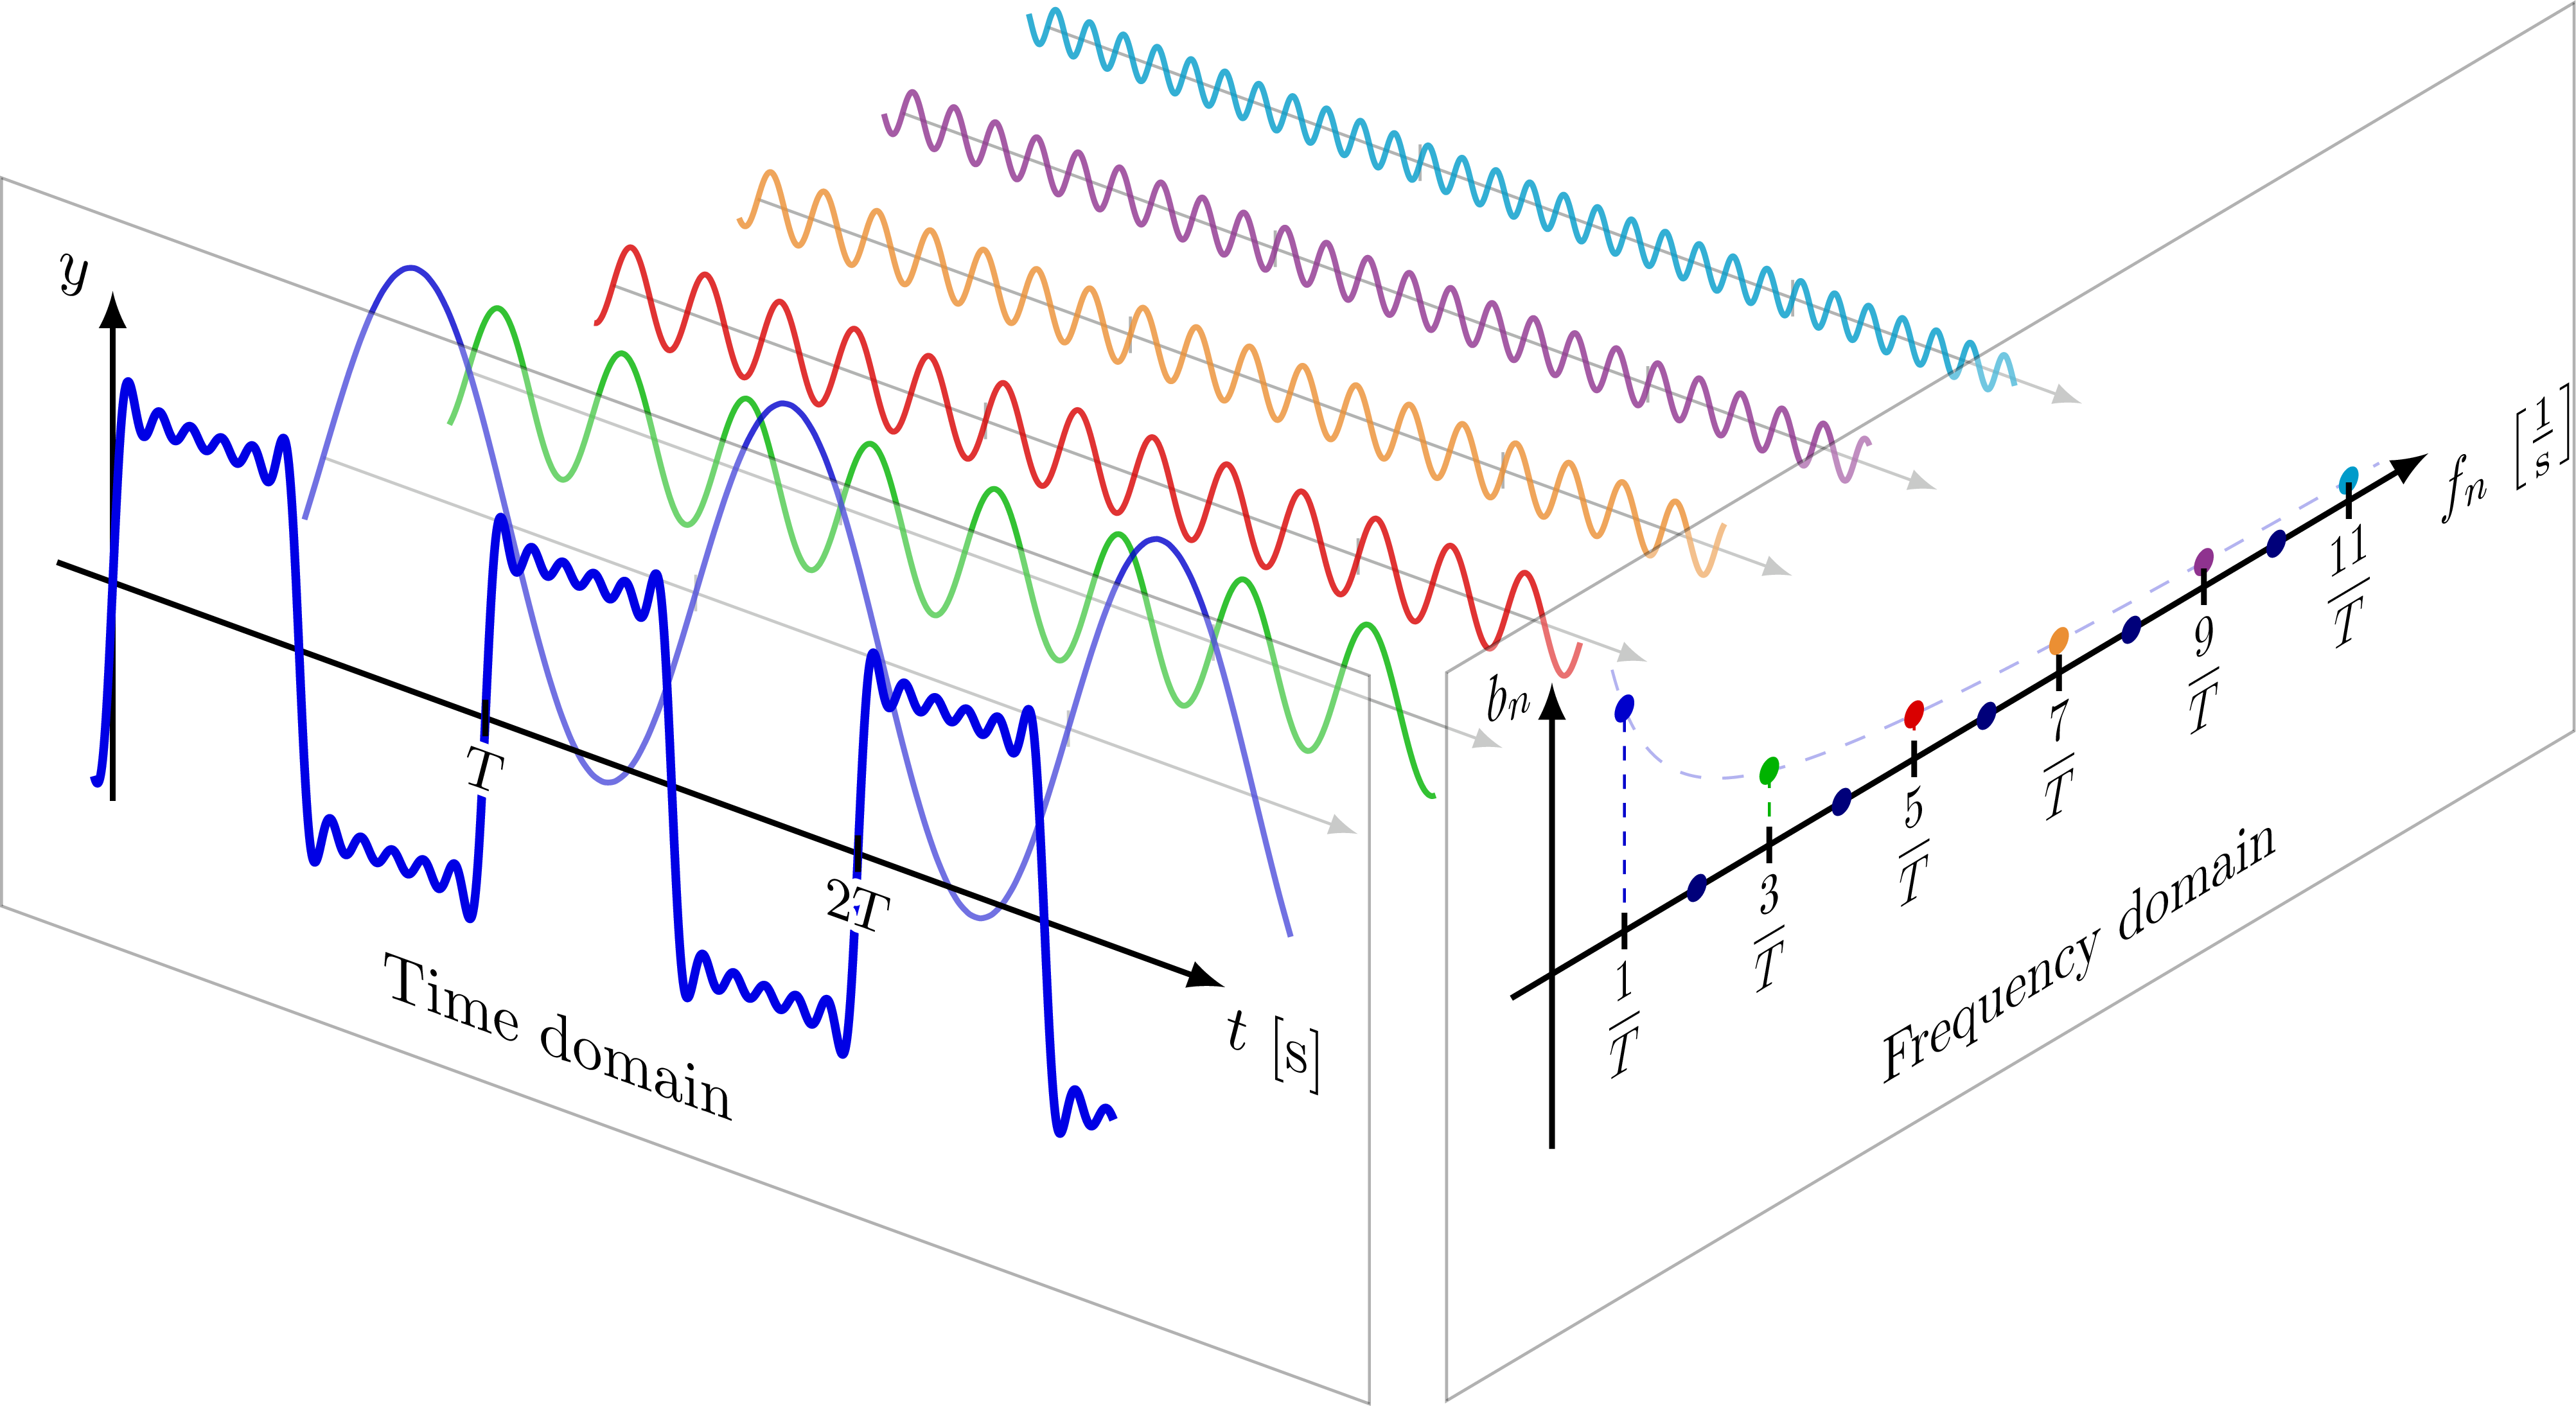
\includegraphics[width=0.9\textwidth]{FourierSeries_Freq.png}
  \caption{Representación visual de la transformada de Fourier \cite{OGorman-2023}.}
  \label{fig:fourier}
\end{figure}

\subsubsection{Espectrogramas}



\subsubsection{Rangos de frecuencias}

\section{Resultados}

\section{Conclusiones}



\begin{thebibliography}{9}
  \bibitem{university-physics}
  H. D. Young and Roger A. Freedman, \emph{University Physics with Modern Physics}, 
  Addison-Wesley, San Francisco, 2012. %%Para citar \cite{university-physics}
  \bibitem{frequencies-wave-sound-pso}
  Al Hwaitat et Al, Journal of Experimental \&\ Theoretical Artificial Intelligence,
  2022, 34, 749-780
  \bibitem{orchestra-frecuency}
  N. Lenssen, \emph{PhD Thesis: Applications of Fourier Analysis to Audio Signal Processing: An Investigation of Chord Detection Algorithms
  }, Claremont University, 2013.

  \bibitem{octave-definition}
  Britannica, https://www.britannica.com/art/octave-music, (accesado 28 Octubre 2024)
  \bibitem{Montenegro-2009}
  A. Montenegro, \textit{CORE}, 2009, \url{https://core.ac.uk/download/pdf/6448967.pdf}
  \bibitem{Bernal-1999}
  J. Bernal, P. Gómez y J. Bobadilla, \textit{Estudios de fonética experimental}, 1999, \textbf{10}, 75-105.
  \bibitem{OGorman-2023}
  L. O'Gorman, \textit{DIBS Methods Meetings}, 2023, \url{https://dibsmethodsmeetings.github.io/fourier-transforms/}
\end{thebibliography}
\end{document}
